\chapter{Introduction}\label{chap:1}
\section{关于空格}\label{空格} 

任意多个空格与一个空格的功能相同。

只有字符后面的空格是有效的,每行最前面的空格被忽略。

单个换行被视作一个空格,连续两个换行表示分段。

~被称作一种不可打断的空格,排版系统不会在这种空格之间换行。不~~~可~~~打~~~断~~~不要停下来~~啊!

西文的逗号、句号和分号等标点后面应该加空格。

汉字后的空格会被忽略。XeLaTeX会自动为汉字和其他内容之间添加空格。

幻影空格,命令\phantom{参数}生成和参数内容一样大小的空格,可以完成一些占位和对齐效果。

\section{简单排版}
使用 ref 命令来引用之前的 label,例如 Section~\ref{chap:1} shows how to use spaces.
Section 可以加 label,figure、subfigure、table 等等都可以加label。如果中英混排的话还是
尽量建议中英文之间打个空格,避免排版的时候有些行 \LaTeX 不知道在哪换行就超宽了。

中文加粗的话一般用模板就可以解决,咱这简易模板缺字体,以英文为例。
This is \textbf{bold text.} Just use Ctrl + B.

\textit{This is italic text,} \emph{this is emphasized text},
and \textit{this is \emph{emphasized text} in italic environment.}

\textcolor{red}{This is red color text.} % depend on \usepackage{color}

\underline{\textcolor{blue}{\textbf{This} \textit{is} blue color text with underline 
pretending to be a URL.}} Oh shit the underline is black!

$a_1=b^2$
转义符\# \{ \} \_ \$ \textbackslash \~{d} \^{A} \^{} \~{}
% ~ 波浪
% # 用在宏定义中
% $ 数学模式符号
% % 注释符号
% ^ 上标符号
% & 表格对齐符号 
% { } 分组符号 
% _  数学模式的下标符号
% \ 宏命令符号
% 若要在正文中使用这些符号,大部分是在前面加\,
% 而\符号是\textbackslash,~符号是\~{},^符号是\^{}。
"zheshisha"\cite{han2019three} oyes.

'"

在这个模板下使用的字体不区分英文的前后引号,想打引号直接输入俩"",中文则需要先后打出前后引号“”。例如~"Hello World!" 和 “哈喽!”

还记得吗,汉字后面的空格会被忽略,所以这里的例如后面加了一个波浪号,否则就是例如 "Hello World!" 没有作用,但是前面的空格是有的,当然这个现象比较少见,一般没有英文标点紧跟着汉字出现的情况吧除了引号,所以要比较小心哦。

hello-world

1--10, $-10+10^2+-\times \div$

pozhehao---fjkdslajk
\section{Figure and table}

\subsection{Figure}
Figure 比较简单,记得加 h,最好的办法就是直接复制下面这段代码,修改文件名和 caption
以及 label 就好啦。
\\  % 强制换行
\begin{figure}[h]
    \centering
    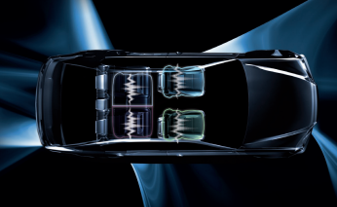
\includegraphics[width=0.7\textwidth]{Img/Chap1/fig1a}
    \caption{This is a car.}
    \label{fig:car}
\end{figure}

subfigure 比较麻烦,实现方法可能会和具体的模板有关。
\begin{figure}[h]
    \centering
    \subfigure[wow]{\label{fig2a}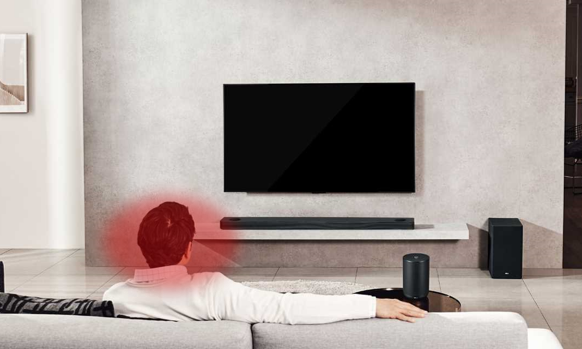
\includegraphics[width=0.31\textwidth]{Img/Chap1/fig1b}}
    ~
    \subfigure[awesome]{\label{fig2b}
\includegraphics[width=0.31\textwidth]{Img/Chap1/fig1c}}
    ~
    \subfigure[]{\label{fig2c}
\includegraphics[width=0.31\textwidth]{Img/Chap1/fig1d}}
    \caption{bla bla. (a): wow, (b): awesome, (c):amazing.}
    \label{fig:bla bla}
\end{figure}

% 在这里要空一行,否则下面这段话会和上面那句话混在一起,你可以试试把上面这个空行删掉就知道啥意思了。
我找到 subfigure 的 caption 在哪加了,在\textbackslash subfigure 后面的方括号里面加!
最终是直接在子图下面加注释还是统一在整个 figure 的 caption 里面加注释,还是要看具体期刊的要求。

\subsection{Table}
表格比较麻烦啦。表格的表头是不是要放在表格上面啊,我刚才忘记讲了,一样先打 caption
后面加 label 就好啦,不过如果这个图表以后不需要引用的话,也可以不加 label。

% See \underline{\textcolor{blue}{http://www.tablesgenerator.com/}}
See \url{http://www.tablesgenerator.com/}

\begin{table}[h]
    \centering
    \begin{tabular}{|lcccc|}    % | 表示竖边框
    \hline      % \hline 表示横边框
       & \textbf{PM-1}  & \textbf{PM-2}  & \textbf{MM}    & \textbf{ACC}   \\
    \hline
    AC & 18.02 & 12.05 & 14.42 & 34.01 \\
    AC & 11.46 & 3.85  & 20.45 & 22.73 \\   % 如果最后有 \hline 这里一定要有 \\
    \hline  
    \end{tabular}
    \caption{这里加表头} % 原来是我们大论文的要求表头放上面,latex默认是放下面的,这里放下面就不会间距太小了
    % 如果你也有放上面的需求就告诉我,其实是可以通过加两行代码解决的!
\end{table}

\textbackslash hline 上面必须有两个斜杠来换行,否则会报错!(除了开头的hline)

\section{Tips}

Ctrl + Alt + B ~~ Build 编译 tex % 我把保存自动编译关了,还是手动按编译比较好!

Ctrl + Alt + V ~~ View  预览 pdf

Ctrl + Alt + J ~~ Jump  跳转至 pdf

Ctrl + left click ~~~~ 跳转至源代码

如果报错了一定不要着急,他出错的地方会用红色波浪线标出来的,首先看看报错信息,如果有
``Missing \}" 类似的话,估计是你忘记加大括回了,如果是 ``Undefined control sequence",
那一定是你用了某个命令,缺少相应的宏包,百度一下宏包叫啥然后 usepackage 就好了。
害还不如你直接喊我就完事了!其实你只需要注重论文的内容,排版什么的可以完全交给我来解决。
所以这个 tex 文件里的技巧应该足够你写论文啦。

最后别忘了在 vscode 中修改 json 文件,在文件-首选项-设置中,在右上角找到 打开设置(json),
打开的 json 文件中如果是空的那就直接把我给你的文件复制粘贴进去,如果已经有内容了,那咱就小心点,
把我们文件中最开头的大括号和最后面的大括回删掉,剩下的粘贴到他的 json 文件的末尾。

对了,你 build 的 pdf 文件在根目录下的 Tmp 文件夹下!

\section{Citation}
在 \textbackslash end\{document\} 之前加上最后这两行, bibliographystyle 是指参考文献的格式,
推荐就用 unsrt 吧,按照引用的先后顺序排序,并且按照数字引用。如果你们专业要求
把参考文献按照作者姓名排序,并且用 authoryear 格式引用,那就改成 apalike。

bibliography 里面是你 .bib 文件的文件名,不用加扩展名\cite{Garzone2002Interpretinginthe,Gentzler2017Translationandrewriting,JinYing2018JiaoTiChuan}。

bib 文件中的每一项长这样:

(见源代码中的注释)
% @book{rayleigh1896theory,
%   title={The theory of sound},
%   author={Rayleigh, John William Strutt Baron},
%   volume={2},
%   year={1896},
%   publisher={Macmillan}
% }

book 是这个文献的类型,rayleigh1896theory 叫做 citekey,是你引用时的入口,从谷歌学术中导出的就是\cite{LiYaShu2017KeXueFan}
作者+年份+title的第一个单词,后面的内容就不介绍了,就是这篇文献的基本信息啦。
bib 文件中千万不能有 citekey 相同的文献,会报错的,我就出现过两次找了半天原来是这里出错了!

想要引用的话直接用 \textbackslash cite 命令就可以了,输入完 cite 直接按 Tab
键可以自动补全大括号(begin 等等后面带大括号的一般都可以),然后输入作者的名字+年份
基本就可以筛选出来了,再次按下 Tab 键可以自动补全剩下的 citekey\cite{Malmkjaer2017TheRoutledgeHandbook,Officer1958Introductiontothe,TanXueLan2019DangDaiYi}。

最后差点忘了,刚才视频里忘记说了,你需要下载一个 Zotero 的插件叫做 Better BibTeX,
安装好后在 Zotero 中的编辑-首选项-Better BibTeX 中找到 Citation key format, 
修改为 [auth][year][Title:split-ideographs:select=1,3],这样软件生成的 citekey 就和
谷歌学术中生成的是差不多的了\cite{WangBinHua2019KouYiLi,XuMing2016YiShiChang},
但是不一致哈哈哈!可以从那导出 bibtex 然后导入到 Zotero 库中,我们再 refresh 一下 citekey 就好了。 Test glossary in this page: \gls{mm}, \gls{atf}.

\section{Glossary}
First use: \gls{acc}, second use: \gls{acc}.

First use: \gls{lcmv}. After the first use, you can just type LCMV if you don't want to show the page numbers in the Glossary List.

And other glossary: \gls{fft}, for the second use: \gls{fft}. \Gls{jpvm} you can get an upper-case full name if it's at the beginning of the sentence. \gls{fft}, \gls{mm}, and \gls{atf}.

Massive testing: \Gls{sfr}, \gls{sfs}, \gls{ft}, \gls{pm}, \gls{pc}, \gls{ift}, \gls{isft}, \gls{ifft}, \gls{aed}, \gls{bc}, \gls{wfs}, \gls{hoa}.

\clearpage % 可以强制分页

